

\tikzset{every picture/.style={line width=0.75pt}} %set default line width to 0.75pt        

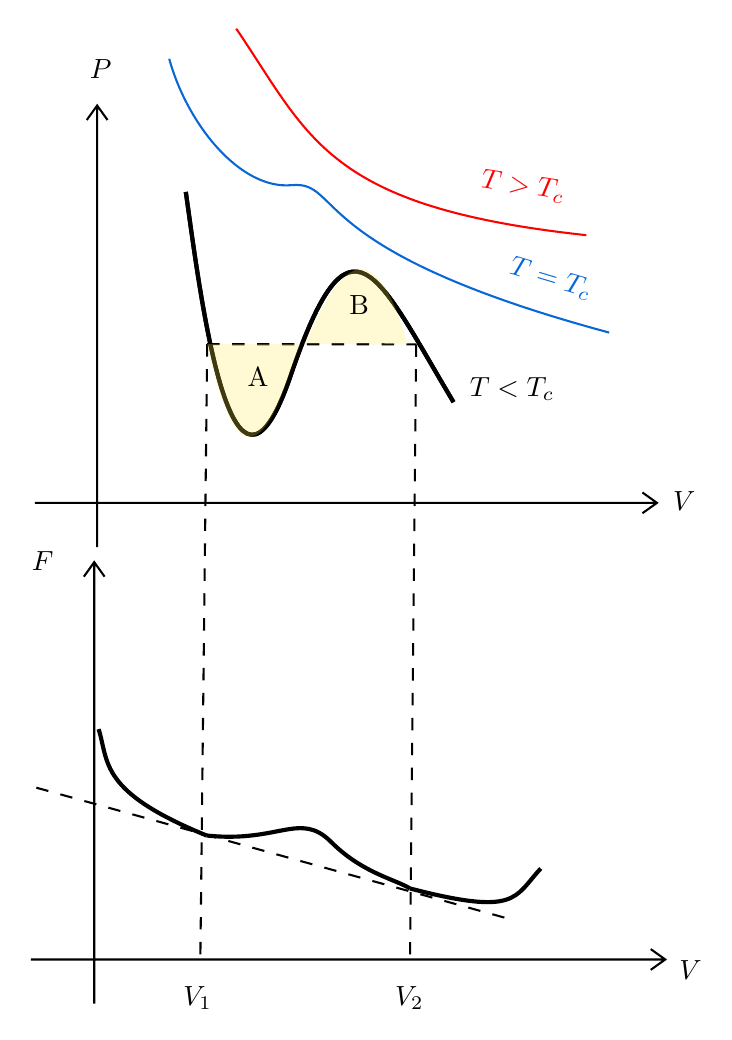
\begin{tikzpicture}[x=0.75pt,y=0.75pt,yscale=-1,xscale=1]
%uncomment if require: \path (0,527); %set diagram left start at 0, and has height of 527

%Shape: Axis 2D [id:dp970091110037609] 
\draw  (51,254.44) -- (350.68,254.44)(80.97,63) -- (80.97,275.72) (343.68,249.44) -- (350.68,254.44) -- (343.68,259.44) (75.97,70) -- (80.97,63) -- (85.97,70)  ;
%Shape: Axis 2D [id:dp5002897351550694] 
\draw  (49,474.44) -- (354.68,474.44)(79.57,283) -- (79.57,495.72) (347.68,469.44) -- (354.68,474.44) -- (347.68,479.44) (74.57,290) -- (79.57,283) -- (84.57,290)  ;
%Curve Lines [id:da45956577782421615] 
\draw [line width=1.5]    (123.68,104.65) .. controls (130.72,153.89) and (145.48,277.34) .. (174.31,192.83) .. controls (203.14,108.32) and (215.68,143.92) .. (252.68,205.92) ;
%Curve Lines [id:da823430407451243] 
\draw [line width=1.5]    (123.68,104.65) .. controls (130.72,153.89) and (145.48,277.34) .. (174.31,192.83) .. controls (203.14,108.32) and (215.68,143.92) .. (252.68,205.92) ;

%Straight Lines [id:da11792893756552392] 
\draw  [dash pattern={on 4.5pt off 4.5pt}]  (134,178) -- (234.68,178.05) ;
%Straight Lines [id:da15895122499938086] 
\draw  [dash pattern={on 4.5pt off 4.5pt}]  (134,178) -- (130.68,475.37) ;
%Straight Lines [id:da8118475157989993] 
\draw  [dash pattern={on 4.5pt off 4.5pt}]  (234.68,178.05) -- (231.68,476.37) ;
%Straight Lines [id:da09683450161007845] 
\draw  [dash pattern={on 4.5pt off 4.5pt}]  (51.68,391.67) -- (278.68,454.67) ;
%Curve Lines [id:da021972733689352486] 
\draw [line width=1.5]    (133.68,414.7) .. controls (168.68,418.45) and (178.68,402.8) .. (193.68,417.8) .. controls (208.68,432.8) and (224.68,435.8) .. (231.68,440.23) ;
%Curve Lines [id:da2284935025874082] 
\draw [line width=1.5]    (231.68,440.23) .. controls (283.68,453.62) and (281.68,444.62) .. (294.68,430.62) ;
%Curve Lines [id:da760370312377808] 
\draw [line width=1.5]    (133.68,414.7) .. controls (81.68,393.45) and (86.68,379.45) .. (81.68,363.45) ;
%Shape: Boxed Bezier Curve [id:dp5322575875876991] 
\draw [color={rgb, 255:red, 255; green, 0; blue, 0 }  ,draw opacity=1 ]   (148,26) .. controls (183.45,78.08) and (190.94,111.93) .. (316.68,125.47) ;
%Shape: Boxed Bezier Curve [id:dp7587016286783995] 
\draw [color={rgb, 255:red, 8; green, 103; blue, 215 }  ,draw opacity=1 ]   (115.68,40.47) .. controls (124.45,72.24) and (149.95,103.61) .. (174.66,101.37) .. controls (199.37,99.14) and (180.24,132.68) .. (327.68,172.4) ;
%Shape: Path Data [id:dp7034407204988964] 
\draw  [draw opacity=0][fill={rgb, 255:red, 255; green, 235; blue, 78 }  ,fill opacity=0.25 ][line width=0.75]  (173.01,193.83) .. controls (155.07,246.42) and (142.57,218.48) .. (134,178) -- (178.77,178) .. controls (176.92,182.72) and (175,187.99) .. (173.01,193.83) -- cycle ;
%Shape: Path Data [id:dp6192702070359754] 
\draw  [draw opacity=0][fill={rgb, 255:red, 255; green, 235; blue, 78 }  ,fill opacity=0.25 ][line width=0.75]  (187.2,165.13) .. controls (207.36,122.74) and (221.19,145.37) .. (230.61,178.1) -- (180.73,177.9) .. controls (182.81,174.09) and (184.96,169.84) .. (187.2,165.13) -- cycle ;

% Text Node
\draw (76,39.4) node [anchor=north west][inner sep=0.75pt]    {$P$};
% Text Node
\draw (357,247.4) node [anchor=north west][inner sep=0.75pt]    {$V$};
% Text Node
\draw (360,473.4) node [anchor=north west][inner sep=0.75pt]    {$V$};
% Text Node
\draw (48,276.4) node [anchor=north west][inner sep=0.75pt]    {$F$};
% Text Node
\draw (265.7,91.6) node [anchor=north west][inner sep=0.75pt]  [color={rgb, 255:red, 255; green, 0; blue, 0 }  ,opacity=1 ,rotate=-8.82]  {$T >T_{c}$};
% Text Node
\draw (280.7,133.44) node [anchor=north west][inner sep=0.75pt]  [color={rgb, 255:red, 8; green, 103; blue, 215 }  ,opacity=1 ,rotate=-16.74]  {$T=T_{c}$};
% Text Node
\draw (259,192.4) node [anchor=north west][inner sep=0.75pt]  [color={rgb, 255:red, 0; green, 0; blue, 0 }  ,opacity=1 ]  {$T<T_{c}$};
% Text Node
\draw (121,486.12) node [anchor=north west][inner sep=0.75pt]    {$V_{1}$};
% Text Node
\draw (223,486.1) node [anchor=north west][inner sep=0.75pt]    {$V_{2}$};
% Text Node
\draw (152,188) node [anchor=north west][inner sep=0.75pt]   [align=left] {A};
% Text Node
\draw (201,153) node [anchor=north west][inner sep=0.75pt]   [align=left] {B};


\end{tikzpicture}
